\documentclass[12pt]{beamer}
\author{Yan Wang}
\title{Paper Reading Seminar}
\subtitle{}
\usetheme{Malmoe}
\setbeamertemplate{navigation symbols}{}
\newcommand*\oldmacro{}%
\let\oldmacro\insertshorttitle%
\renewcommand*\insertshorttitle{%
\oldmacro\hfill%
\insertframenumber\,/\,\inserttotalframenumber}

\begin{document}

\begin{frame}[plain]
    \titlepage
\end{frame}

\begin{frame}{Image Matching via Saliency Region Correspondences}
    \begin{itemize}
        \item Intuition
        \begin{itemize}
            \item Segmentation is not perfect. Weak connections $\Rightarrow$ graph-based segmentation (NCut)
            \item Matching is not perfect. Weak connections $\Rightarrow$ spatial consistency check
            \item Combine the two tasks together $\Rightarrow$ use a single graph to get a joint optimal
            \item Encoding context in the matching process $\Rightarrow$ no need for spatial consistency check
        \end{itemize}
        \item Outline
        \begin{itemize}
            \item Formulation
            \item Optimization
            \item Features
        \end{itemize}
    \end{itemize}
\end{frame}

\begin{frame}{Formulation}
    \begin{itemize}
        \item Graph formulation
        \begin{itemize}
            \item Vertex: pixel
            \item Layer: two-layer, one for each image
            \item Intra-layer edges: how strongly the pixels are similar (connected) in this image
            \item Inter-layer edges: how strongly the pixels are similar (connected) across images
            \\ \medskip { 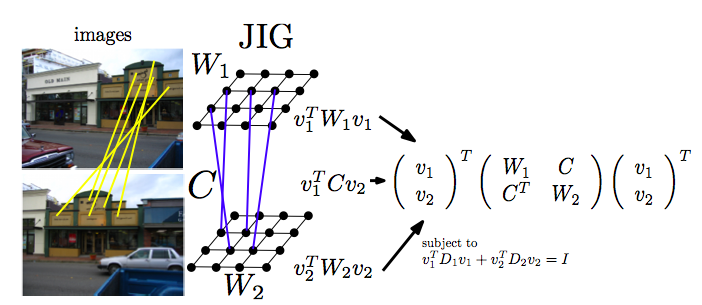
\includegraphics[width=0.7\textwidth]{graph-framework.png} \\ } 
        \end{itemize}
    \end{itemize}
\end{frame}

\begin{frame}{Formulation}
    \begin{itemize}
        \item Intra-layer optimization goal
        \[\max_v \frac{v_1^TW_1v_1 + v_2^TW_2v_2}{v^TDv}\]
        \begin{itemize}
            \item Each segment should be internally consistent $\Rightarrow v_1^TW_1v_1$. Only if $v_{1j}, v_{1k}$ both positive, will $W_{1(i,j)}$ be counted
            \item $v_{ij} = \{0, 1\}^{n_i}, \sum_j v_{ij} = 1$, indicator vector for image $i$, pixel $j$, and cluster $k$, $v = [v_1^T, v_2^T]^T$
            \item Normalize on the size: $\sum_j v_{1j}^TW_1$ = ${\bf 1}^TW_1 = D_1$
        \end{itemize}
    \end{itemize}
\end{frame}

\begin{frame}{Formumation}
    \begin{itemize}
        \item Inter-layer optimization goal
        \[\max_v \frac{v_1^TCv_2}{v^TDv}\]
        \begin{itemize}
            \item ``Co-saliency'' regions (where $v_{ij} = v_{ik}$) should be similar
            \item Also normalize on size
            \item Use ``context'' to refine segmentation as well as matching
        \end{itemize}
    \end{itemize}
\end{frame}

\begin{frame}{Formulation and optimization}
    \begin{itemize}
        \item Final optimization goal
        \begin{itemize}
        \[F(v, C) = \text{IntraIS}(v, C) + \text{InterIS}(v, C)\]
            \item Note $C$ (matching) will affect segmentation result $v$
        \end{itemize}
        \item Relaxation for optimizaiton
        \begin{itemize}
            \item $v$ to real vector
            \item EM iterative optimization (details not read)
        \end{itemize}
    \end{itemize}
\end{frame}

\begin{frame}{Features}
    \begin{itemize}
        \item MSER detector + SIFT descriptor
        \item Intra-image $W$
        \begin{itemize}
            \item $x, y$ are considered in the same segment $\Leftrightarrow$ no edges with large magnitude spatially separate them
            \item Edge detection with large magnitude $\Rightarrow$ get $W$
        \end{itemize}
        \item Inter-image $C$
        \begin{itemize}
            \item 1. Feature detection: also consider the ellipse (orientation/scale) from the detector
            \item 2. Feature matching
            \item 2.0 Simplest pixel-wise matching: Gaussian kernel + descriptor + ellipse matrix
            \[m_{x, y}(p, q) = e^{-\lVert d_p - d_q \rVert^2/\sigma_i^2}e^{-\lVert H_p(x)-H_q(y)\rVert^2/\sigma_p^2}\]
        \end{itemize}
    \end{itemize}
\end{frame}

\begin{frame}{Features}
    \begin{itemize}
        \item Inter-image $C$
        \begin{itemize}
            \item 2. Feature matching
            \item 2.1 Adopt patch-wise feature matching score as pixel-wise score for $C$
            \[M_{x, y} = \max\{m_{x, y}(p, q) \ | \ p\in P, q \in Q, x \in R_p, y \in R_q\}\]
            \item 2.2 Compute patch-wise similarity matrix $M$, and then normalize to $C$
            \[D^{-1/2}_1CD^{-1/2}_2 = P \circ M\]
            (Not really understanding this... They use MSER detector to extract sparse interest points, why can they still get a dense matching score?)
        \end{itemize}
    \end{itemize}
\end{frame}

\begin{frame}{Distributed Computer Vision Algorithms Through Distributed Averaging}
    \begin{itemize}
        \item Intuition: make linear algebra algorithms distributed + CV applications
        \item Outline
        \begin{itemize}
            \item Basic distributed algorithms
            \item Linear algebra algorithms
            \item Applications in CV
        \end{itemize}
    \end{itemize}
\end{frame}

\begin{frame}{Basic distributed algorithm}
    \begin{itemize}
        \item Basic assumption
        \begin{itemize}
            \item Several computation nodes with limited computation power as well as battery
            \item Not fully connected: info can only propagated among neighbors
            \\ \medskip { 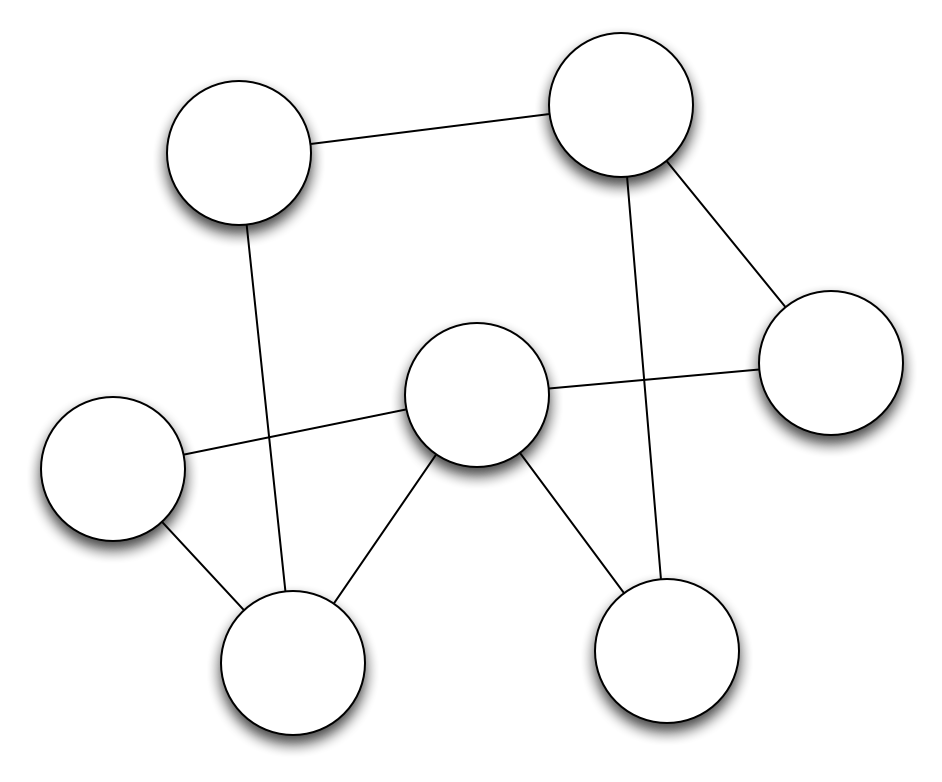
\includegraphics[width=0.4\textwidth]{framework.png} \\ } 
        \end{itemize}
    \end{itemize}
\end{frame}

\begin{frame}{Basic distributed algorithm}
    \begin{itemize}
        \item Averaging a number $x$
        \begin{itemize}
            \item Iterative algorithm: averaging among neighbors
            \[x(t+1) = x(t) + \epsilon \sum_{j \in N_i} \Big(x_j(t) - x_i(t)\Big)\]
            \\ \medskip { 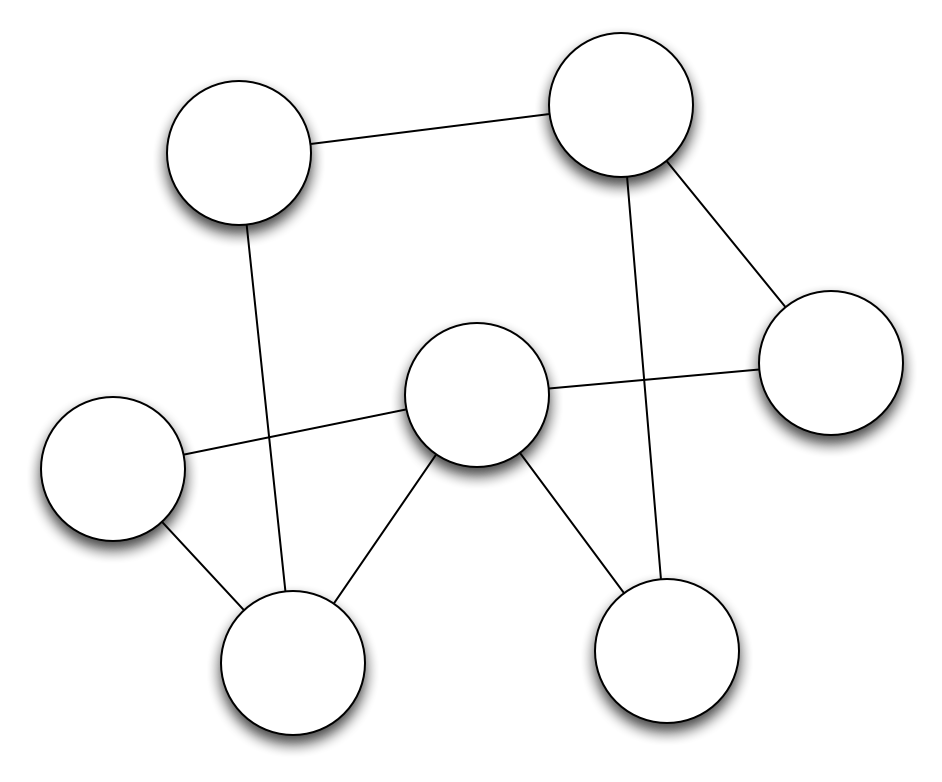
\includegraphics[width=0.4\textwidth]{framework.png} \\ } 
            \item Easily extended to vectors/matrices
        \end{itemize}
    \end{itemize}
\end{frame}

\begin{frame}{Basic distributed algorithm}
    \begin{itemize}
        \item Get the min/max
        \[x_i(t+1) = \min_{j \in \{N_i \bigcup i\}} x_j(t)\]
        \item Covariance
        \begin{itemize}
            \item $A = \begin{bmatrix}A_1^T & A_2^T & \cdots & A_N^T\end{bmatrix}^T \in \mathbb{R}^{n \times m}$
            \item Compute $C = \frac{1}{N}A^TA$
            \[C = \frac{1}{N}\sum_iA_i^TA_i\]
            \item Compute $C_i = A_i^TA_i$, and then average among all the nodes
            \item Only meaning for when rank$(C) \ll n$
        \end{itemize}
    \end{itemize}
\end{frame}

\begin{frame}{Linear algebra algorithms}
    \begin{itemize}
        \item SVD
        \[A = U \Sigma V^T \]
        \begin{itemize}
            \item Compute $C = A^TA$
            \item Locally compute C's SVD: $C = V(\frac{1}{N}\Sigma^2)V^T$
            \item Recover $U_i$ locally: $U_i = A_iV\Sigma^{-1}$
        \end{itemize}
    \end{itemize}
\end{frame}

\begin{frame}{Linear algebra algorithms}
    \begin{itemize}
        \item PCA
        \begin{itemize}
            \item Compute the average of $A$ $\Rightarrow$ do data centralization
            \item Compute covariance matrix $C = A^TA$
            \item Local SVD decomposition: $C = U\Sigma U^T \Rightarrow$ get the basis
            \item Compute the new representation: $\hat{A} = A^TU$
        \end{itemize}
    \end{itemize}
\end{frame}

\begin{frame}{Linear algebra algorithms}
    \begin{itemize}
        \item Least square estimation
        \begin{itemize}
            \item $x_0 = \arg \min_x \lVert Ax - b\rVert^2$
            \item $x_0 = \arg \min_x \lVert A^TAx - A^Tb \rVert^2 $ (is this true?)
            \item $A^TA$ and $A^Tb$ easy to compute distributedly
            \item Can be solved locally
            \item (Not very clear)
        \end{itemize}
    \end{itemize}
\end{frame}

\begin{frame}{Applications in CV}
    \begin{itemize}
        \item Point triangulation
        \item Linear pose estimation
        \item Structure from Motion
    \end{itemize}
\end{frame}


\begin{frame}{Coherency Sensitive Hashing}
    \begin{itemize}
        \item A simple introduction
        \item Find ANN for local patches
        \item Naive baseline: brute-force match in the feature space
        \item PatchMatch: like Genetic Algorithm
        \begin{itemize}
            \item Hold a candidate pool
            \item If two patches in two images are similar, include nearby patches in the pool
            \item Randomly add patch pairs in the pool to get rid of (too) local minima.
        \end{itemize}
    \end{itemize}
\end{frame}

\begin{frame}{Approach}
    \begin{itemize}
        \item Hashing + more sophisticated candidate expansion
        \begin{itemize}
            \item Hashing: LSH + 2D Walsh Hadamard Kernel
            \item Candidate expansion
            \begin{itemize}
                \item $g_A(a) = g_B(b) \Rightarrow $ include $b$ in Cand($a$)
                \item $b \in \text{Cand}(a_1), g_A(a_1) = g_A(a_2) \Rightarrow$ include $b$ in Cand($a_2$)
                \item $b_1 \in \text{Cand}(a_2), g_B(b_1) = g_B(b_2) \Rightarrow$ include $b_2$ in Cand($a_2$)
                \item Include spatial neighbor pairs in the candidates
            \end{itemize}
            \item Still need to do verifications on the candidate set
        \end{itemize}
    \end{itemize}
\end{frame}

\end{document}

